\documentclass{article}
\usepackage[pdfcreator={LaTeX}]{hyperref}
\usepackage{graphicx}
\usepackage[utf8]{inputenc} 
\usepackage[ngerman]{babel}


\usepackage{tikz}
\usetikzlibrary{arrows,shadows}
\usepackage{pgf-umlsd}


\begin{document}
\begin{titlepage}

\begin{center}
\textbf{\textsc{\LARGE Entwurf}}

{\large \today}

\vspace{2cm}
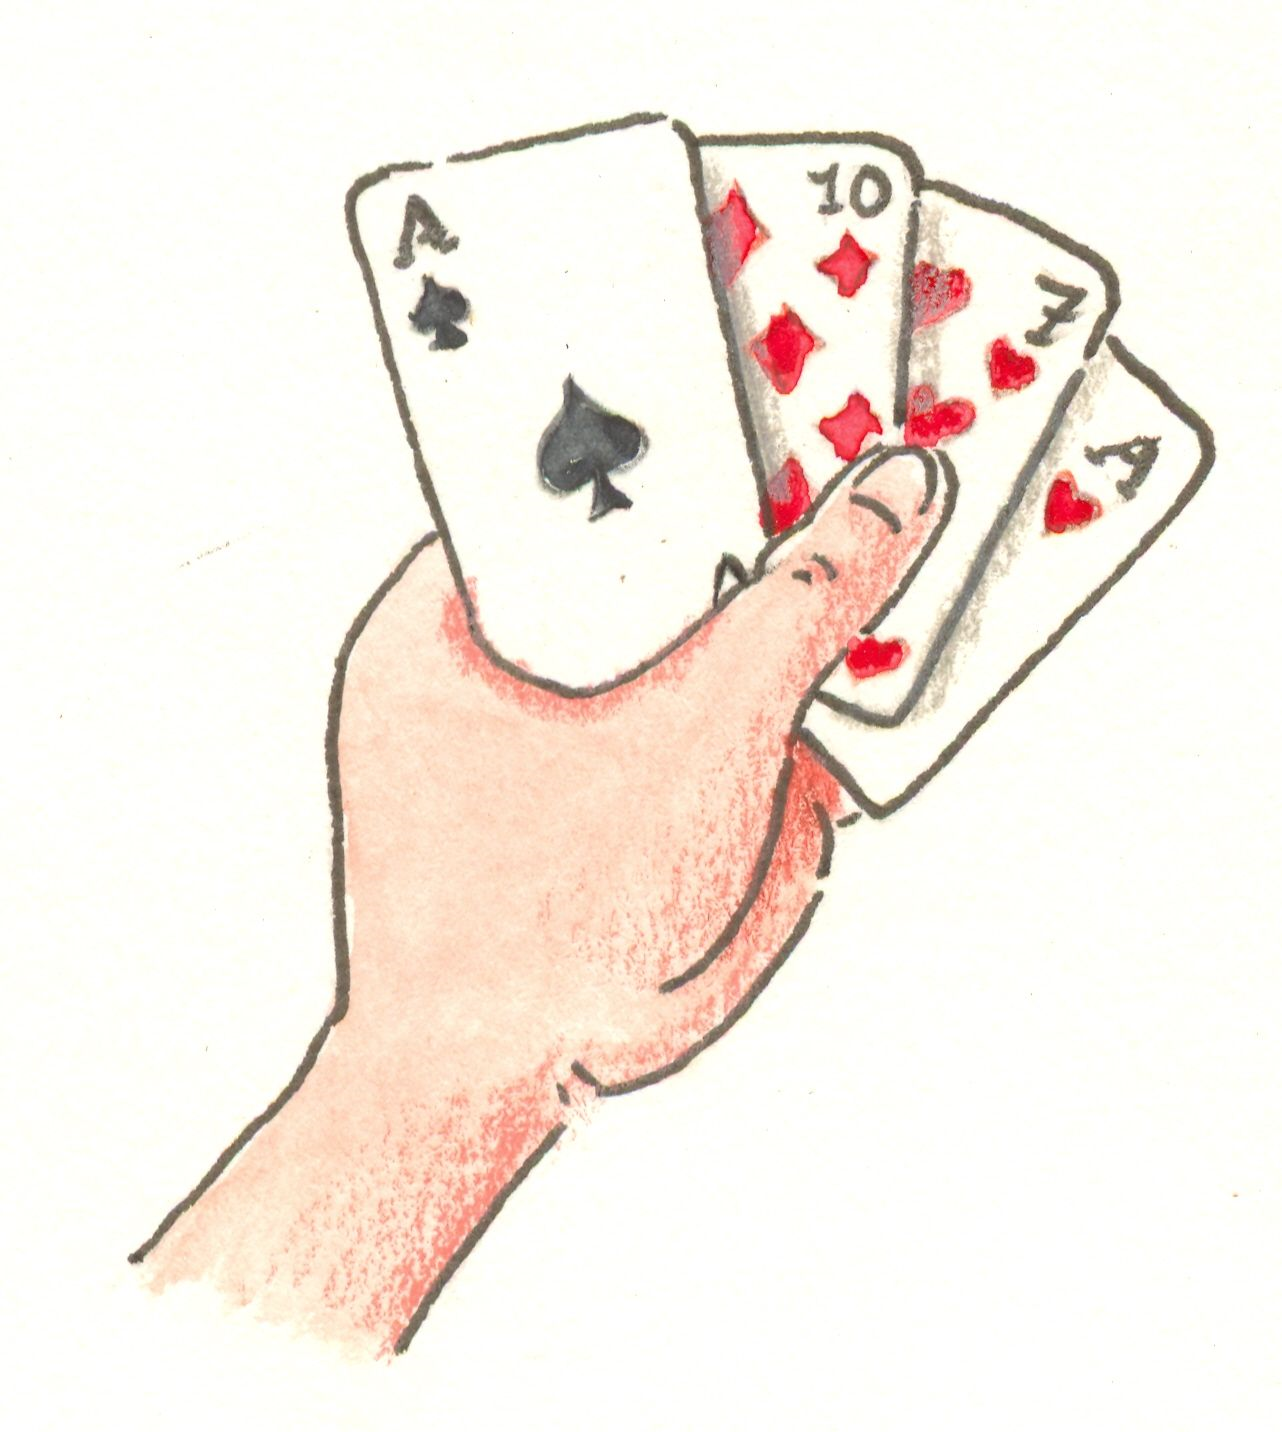
\includegraphics{kartenspiel}
\ \\
\ \\

\textbf{\textsc{\LARGE NET-WizHearts}}
\vspace{2cm}

\begin{tabular}{|c|c|c|}\hline
   Phase & Verantwortlicher & E-Mail \\ \hline\hline
   Pflichtenheft & Alina  Meixl  &  alina@meixl.de \\ \hline
   Entwurf & Viktoria Witka & witkaviktoria@freenet.de \\ \hline
   Spezifikation & Daniel Riedl & dariedl14@yahoo.de \\ \hline
   Implementation & Andreas Altenbuchner& a.andi007@gmail.com\\ \hline
   Verifikation &Patrick Kubin & kubin@fim.uni-passau.de\\ \hline
   Präsentation & w& w\\ \hline
 \end{tabular}

\end{center}

\end{titlepage}


\tableofcontents
\newpage

\section{Einleitung}
-----Achtung Kopie -------
In diesem Dokument wird der konzeptionelle Entwurf des Online Multiplayer Kartenspiels NET-WizHearts dargestellt.\\
\ \\
Es wird eine erste Übersicht über die verschiedenen Komponenten des MVC-
Modells, das der Anwendung zugrunde liegt, gegeben. Dies geschieht durch eine
Angabe der Klassenstruktur. Einzelne Funktionsaufrufe
werden beispielhaft zu Illustrationszwecken in Sequenzdiagrammen dargestellt.\\
\ \\
Durch das Verwenden des MVC Design Patterns wird eine Unabhängigkeit der View-Schicht 
vom restlichen System erzielt, so dass die graphisch Oberfläche - wie gefordert - ohne Anpassung 
der Modell- und Controllerschicht auch für andere Regelwerke einsetzbar ist.\\
\  \\
WEITERES


\section{Architektur-Diagramm}
Client-Server Diagramm. Client hat MVC Architektur.
\  \\
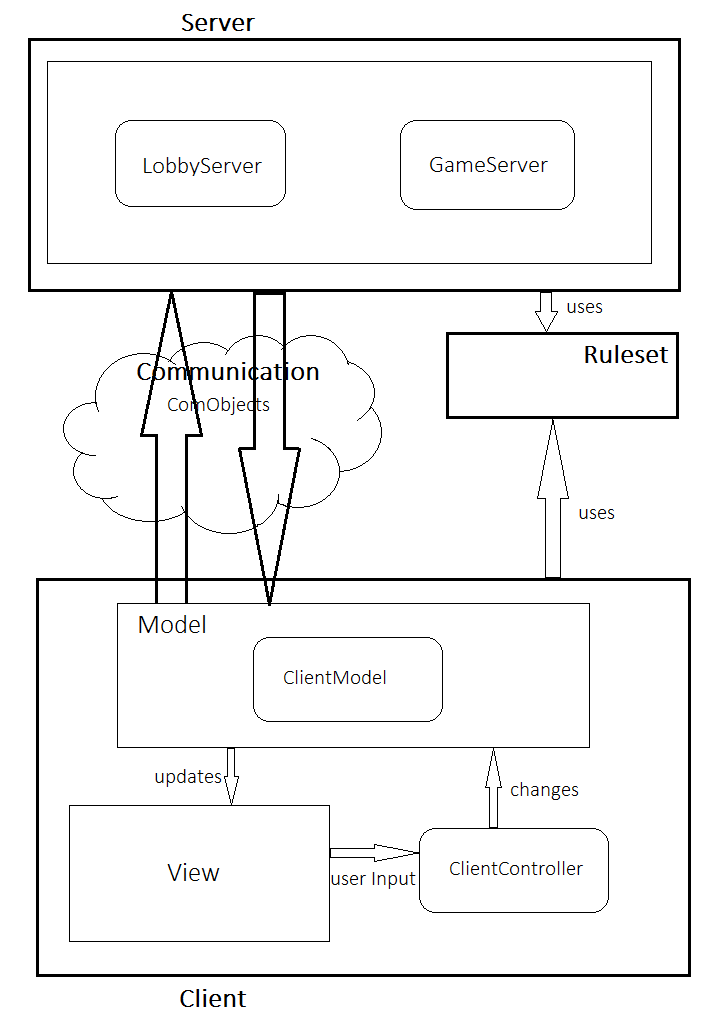
\includegraphics[height=15cm]{ArchitekturDiagramm}
\newpage
\section{Klassendiagramm}
\subsection{Packages}
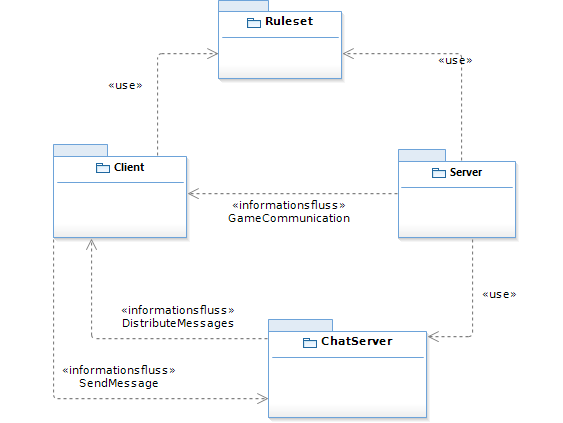
\includegraphics[width=\textwidth]{Packages}
\subsection{Server}
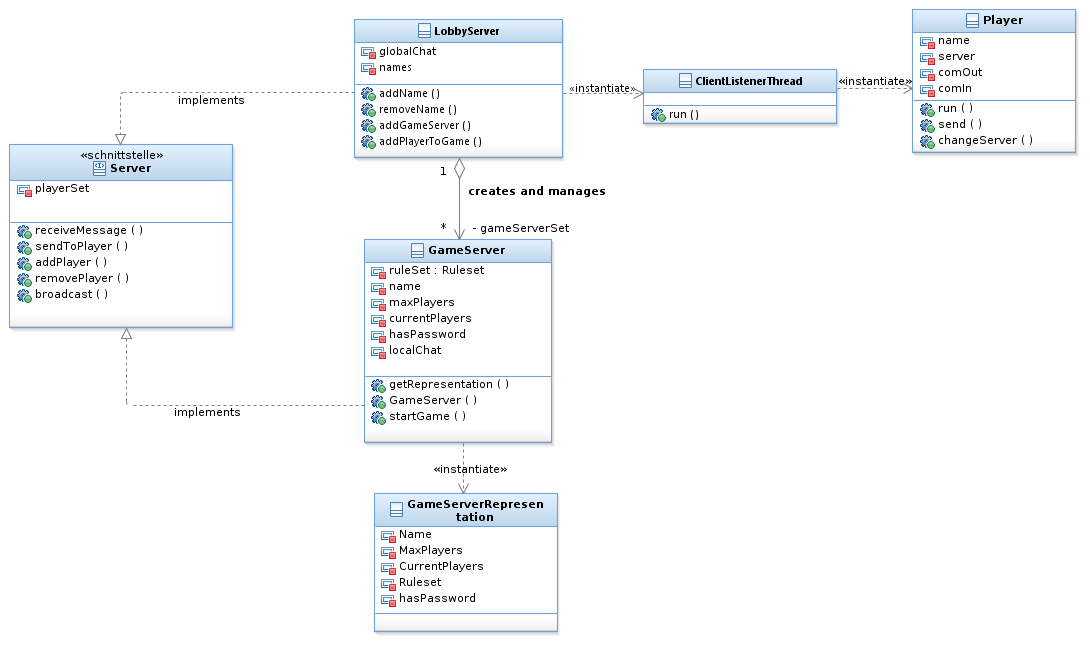
\includegraphics[width=\textwidth]{Server}
\subsection{ChatServer}
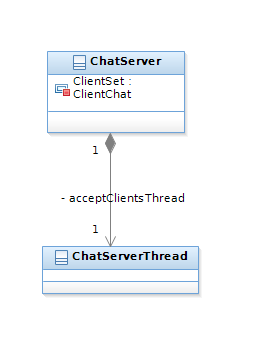
\includegraphics[width=5cm]{ChatServer}
\subsection{Client}
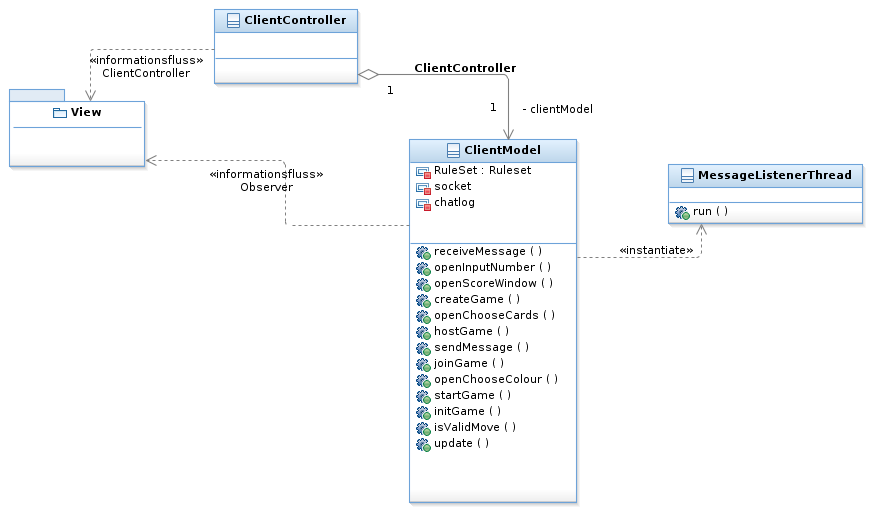
\includegraphics[width=\textwidth]{Client}
\subsection{ClientView}
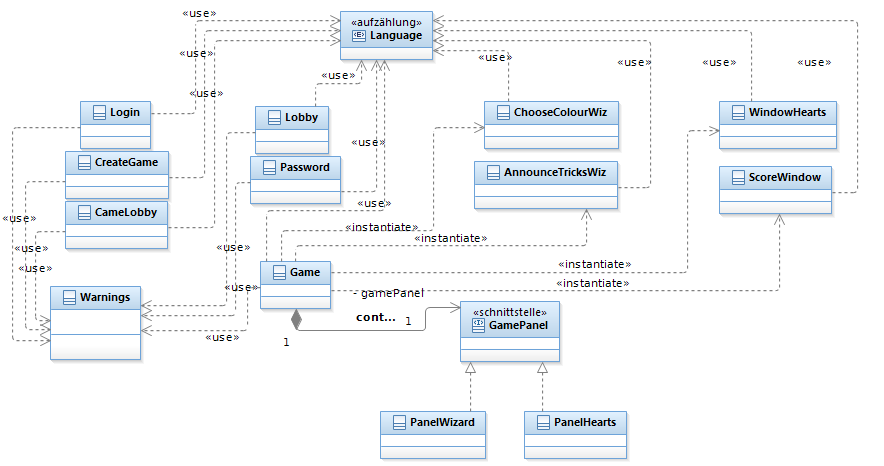
\includegraphics[width=\textwidth]{ClientView}
\subsection{Ruleset}
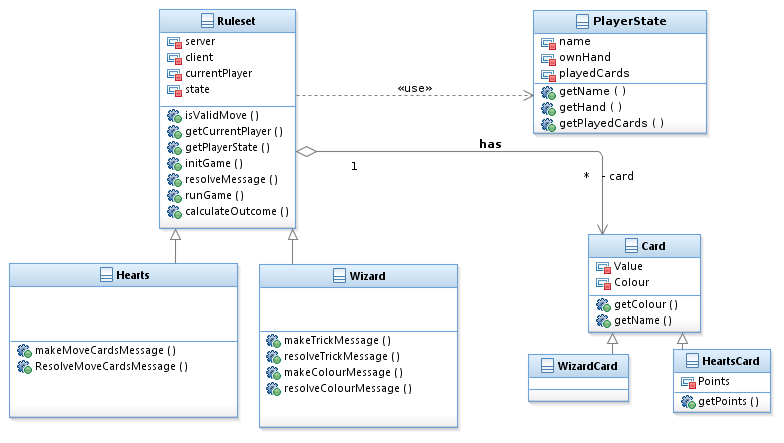
\includegraphics[width=\textwidth]{Ruleset}

\ \\
\section{Klassenbeschreibung}
Wichtigste Klassen und ihr Verwendungszweck.
	\subsection{Server}
		\subsubsection{Server}
			\textbf{Server} erstellt neue Spiele und ist sowohl für die Verwaltung aller Spiele, als auch der Spieler und dem Chatroom in der Lobby, zuständig. \\
			\textbf{Serverthread} verwaltet die einzelnen Threads vom Server. \\
			\textbf{GameServer} verwaltet ein Spiel, ihre Spieler, sowie den Chatroom im Spiel und überprüft die Einhaltung der Regeln in jedem Zustand. \\
			\textbf{Gamestate} repräsentiert einen bestimmten  Spielzustand welches vom Regelwerk ausgewertet werden kann.\\
			\textbf{Player} repräsentiert einen Client, enthält den Namen des Clients und verwaltet die Ein- und Ausgänge seiner Socketverbindung. \\
		\subsubsection{Chatserver}
			\textbf{Chatserver} verwaltet die Kommunikation zwischen Spielern in einem Chatroom, bei einem Spiel werden auch Ereignisse ausgegeben. \\
			\textbf{ChatServerThread} verwaltet die einzelnen Threads vom Chatserver.
	\subsection{Ruleset}
		\textbf{Ruleset} ist eine abstrakte Klasse welches zu einem Spiel die Regeln und den Ablauf bestimmt. Außerdem überprüft es ob jeder neuer Spielzustand regelkonform ist. \\
		\textbf{Hearts} erstellt das Regelwerk zum Spiel Hearts. \\
		\textbf{Wizard} erstellt das Regelwerk zum Spiel Wizard. \\
		\textbf{Card} ist eine abstrakte Klasse und repräsentiert eine Karte. Jede Karte besitzt als Attribute einen Wert und eine Farbe. \\
		\textbf{HeartsCard} repräsentiert eine Karte aus dem Spiel Hearts. \\
		\textbf{Wizard} repräsentiert eine Karte aus dem Spiel Wizard.
	\subsection{Client}
	\subsubsection{Model}
		Startklasse \\
		Serververbindung(F040)\\
		Benutzername prüfen, speichern(F040)\\
		Spracheinstellungen(F050W) \\
		Regeln überprüfen(erlaubte züge, welcher Spieler ist dran etc.)\\
		Spielstand verwalten \\
		Punktestand verwalten\\
		Chatnachrichten senden und empfangen(Spiel, Lobby, Wartefenster) \\
		Lobby	verwalten (Spiel erstellen, beitreten, löschen, verlassen)\\	
		Erstellungsfenster verwalten (Passwort, regelwerk, spielname)\\
		Wartefenster(Spieler löschen,verlassen)
		Passwortabfrage(vergleich)\\
	\subsubsection{Controller}
	\subsubsection{View}
			\textbf{Login} repräsentiert den initialen Dialog indem der Benutzer seinen Namen und die Adresse des Servers eingeben kann. Außerdem ist über den Login die Auswahl der Sprache möglich.\\
			\textbf{Lobby} erzeugt die Ansicht der ServerLobby. Es können offene Spiele und Spieler betrachtet sowie gechattet werden. \\
			\textbf{CreateGame} bietet alle Komponenten um ein Regelwerk zu wählen, einen Spielnamen fest zulegen und das Spiel durch ein Passwort zu schützen. \\
			\textbf{Password} ermöglich die Eingabe eines Passwortes um einem geschlossenem Spiel beizutreten. \\
			\textbf{GameLobby} modelliert das Wartefenster indem beigetretene Spieler auf den Start des Spieles durch den Spielleiter warten. \\
			\textbf{Game} ist der allgemeine Teil des Spielfensters der den Chat beherbergt. \\
			\textbf{PanelWizard} ist die für das Spiel Wizards angepasste Teilkomponente des Spielfensters. \\
			\textbf{PanelHearts} ist die für das Spiel Hearts angepasste Teilkomponente des Spielfensters. \\
			\textbf{Warnings} gibt Dialoge aus, die dem Spieler Fehlermeldungen und Hinweise geben. \\
			\textbf{ChooseColourWiz} ermöglicht es Spielern in einer Partie Wizards die Trumpffarbe auszuwählen. \\
			\textbf{AnnounceTricksWiz} erstellt ein Fenster mit dessen Hilfe man zu beginn einer Runde Wizards seine Stiche tippen kann. \\
			\textbf{WindowHearts} erzeugt ein Fenster zu beginn einer Partie Hearts über das Karten zu anderen Spielern weitergereicht werden müssen. \\
			\textbf{ScoreWindow} zeigt den Punktestand nach einem Spiel an.\\

\section{Sequenzdiagramme}
	\subsection{Spielstart}
		Mr. Blue, Mr. White und Mr.Pink befinden sich in der Lobby. \\
		Mr. Blue klickt auf 'New Game' und wird ins Erstellungsfenster geschickt. \\
		Er nimmt die nötigen Einstellungen vor(z.B Wizard auswahlen, Name setzen) und druckt auf 'Create'. Er wird ins  Wartefenster weitergeleitet.\\
		Mr. Pink und Mr. White wählen Mr. Blues spiel in der Lobby aus und drücken auf 'Join'. Sie werden an die Passwortabfrage geschickt.\\
		Sie geben das Passwort ein und werden ans Wartefenster geschickt.\\
		Die Mindestanzahl von drei ist erreicht. Mr. Blue drückt auf 'Start Game'.\\
		Mr. Blue, Mr. Pink und Mr. White werden ins Spiel geschickt. Das Spiel startet.\\


\newpage
\setlength{\hoffset}{-30mm}
\setlength{\topmargin}{-3.0cm}
\begin{sequencediagram}

\newthread[white]{b}{B}
\newinst[0.1]{w}{W}
\newinst[0.1]{p}{P}
\newinst[0.1]{l}{Lobby}
\newinst[0.1]{e}{CreateG.}
\newinst[0.1]{g}{GLobby}
\newinst[0.1]{a}{Game}
\newinst[0.1]{c}{CModel}
\newinst[0.1]{s}{Server}
\newinst[0.1]{gs}{GServer}

\mess{b}{klicknewGame}{l}	
\begin{call}{l}{newGame()}{c}{}
	\begin{call}{c}{close()---Lobby Mr.Blue}{l}{}	
	\end{call}	
	\mess{c}{toCrGameMrBlue}{s}	
	\mess{s}{removePlayerMrBlue}{c}			
	\begin{call}{c}{removePlayer(Mr.Blue)}{l}{}	
	\end{call}
	\begin{call}{c}{open()--- Mr.Blue}{e}{}
		\mess{b}{RulesetWizard,Name,Create}{e}
		\begin{call}{e}{openGame()}{c}{}	
		\end{call}		
	\end{call}
	\begin{call}{c}{close()}{e}{}	
	\end{call}
	\begin{call}{c}{open()--- Mr.Blue}{g}{}
			\mess{c}{newGameMrBlue}{s}
			\begin{call}{s}{newGameServer(Mr.Blue,Wizard, 'MrBluesGame')}{gs}{}				
				\mess{s}{openedGameMrBlue}{c}
				\begin{call}{c}{addOpenedGame(Mr.BluesGame, Wizard)}{l}{}
					\mess{b}{Hier 2te Seite}{l}
				\end{call}
			\end{call}
		\end{call}	
\end{call}	

\end{sequencediagram}
\newpage
\setlength{\hoffset}{0mm}
\setlength{\topmargin}{0cm}
	
\newpage
\setlength{\hoffset}{-30mm}
\setlength{\topmargin}{-3.0cm}
\begin{sequencediagram}

\newthread[white]{b}{B}
\newinst[0.1]{w}{W}
\newinst[0.1]{p}{P}
\newinst[0.1]{l}{Lobby}
\newinst[0.1]{e}{CreateG.}
\newinst[0.1]{g}{GLobby}
\newinst[0.1]{a}{Game}
\newinst[0.1]{c}{CModel}
\newinst[0.1]{s}{Server}
\newinst[0.1]{gs}{GServer}
\mess{w}{klickOpenGameMrBluesGame}{l}
	\begin{call}{l}{joinGame(MrWhite)}{c}{}
		\begin{call}{c}{close()---Lobby Mr.White}{l}{}	
		\end{call}	
		\mess{c}{WjoinMrBlue}{s}	
		\begin{call}{s}{addToPlayer(Mr.White)}{gs}{}	
		\end{call}
		\mess{s}{removePlayerMrWhite}{c}
		\begin{call}{c}{removePlayer(Mr.White)}{l}{}	
		\end{call}
		\begin{call}{c}{join()--- Mr.White}{g}{}
		\end{call}
	\end{call}
\mess{p}{klickOpenGameMrBluesGame}{l}
	\begin{call}{l}{joinGame(MrPink)}{c}{}
		\begin{call}{c}{close()---Lobby Mr.Pink}{l}{}	
		\end{call}	
		\mess{c}{WjoinMrBlue}{s}	
		\begin{call}{s}{addToPlayer(Mr.Pink)}{gs}{}	
		\end{call}
		\mess{s}{removePlayerMrPink}{c}
		\begin{call}{c}{removePlayer(Mr.Pink)}{l}{}	
		\end{call}
		\begin{call}{c}{join()--- Mr.Pink}{g}{}
		\end{call}
	\end{call}
	\mess{b}{startGame}{g}
	\begin{call}{g}{goToGame()}{c}{}
	\end{call}
	\begin{call}{c}{close()}{g}{}	
	\end{call}
	\begin{call}{c}{open()}{a}{}
	\end{call}

\end{sequencediagram}
\newpage
\setlength{\hoffset}{0mm}
\setlength{\topmargin}{0cm}


	\subsection{Spielzug}
		Aufgabe: Ein Spieler ist im Spiel Wizard an der Reihe und spielt eine Karte aus.
		Das Diagramm endet sobald der Spielzug auf allen Clients sichtbar
		geworden ist und der nächste Spieler seinen Zug machen kann.\\
		\ \\
		Mr. Blue, Mr. White und Mr.Pink sind im Spiel Wizard. \\
		Mr. Blue ist an der Reihe, wahlt eine Karte durch einmaliges anklicken aus und spielt sie durch ein weiteres anklicken.\\
		Der Zug wird auf Regelkonformität überprüft.\\
		Er ist nicht regelwidrig, also wird die gepielte Karte über den Server verschickt und bei Mr. Blue, Mr. Pink und Mr. White auf dem 	Ablagestapel angezeigt. \\
		Es wird überpruft, wer als nächstes dran ist.\\
		Der nächste Spieler ist am Zug \\

\newpage
\setlength{\hoffset}{-30mm}
\setlength{\topmargin}{-3.0cm}
\begin{sequencediagram}
\newthread[white]{b}{Mr.B}
\newinst[0.3]{g}{Bs Game}
\newinst[0.3]{w}{Ws Game}
\newinst[0.3]{p}{Mr. Ps Game}
\newinst[0.3]{c}{ClientCon.}
\newinst[0.3]{m}{ClientMod}
\newinst[0.3]{rc}{RWClient}
\newinst[0.3]{gs}{GServer}
\newinst[0.3]{rs}{RWServer}

\mess{b}{klickCardTwice}{g}
\begin{call}{g}{playCard()}{c}{}
	\begin{call}{c}{checkRulesLocal(Card)}{m}{true}
		\begin{call}{m}{checkRulesLocal(Card)}{rc}{true}
		\end{call}
	\end{call}
	\begin{call}{m}{checkRulesGlobal(Card)}{gs}{true}
		\begin{call}{gs}{checkRulesGlobal(Card)}{rs}{true}
		\end{call}
	\end{call}

	\begin{call}{gs}{playedCard(Card)}{m}{}
		\begin{call}{m}{update()}{g}{}
		\end{call}
		\begin{call}{m}{update()}{w}{}
		\end{call}
		\begin{call}{m}{update()}{p}{}
		\end{call}
	\end{call}

	\begin{call}{m}{checkNextPlayer()}{m}{}
	\end{call}
	\begin{call}{m}{notifyNextPlayer()}{w}{}
	\end{call}
\end{call}

\end{sequencediagram}
\newpage
\setlength{\hoffset}{0mm}
\setlength{\topmargin}{0cm}			
\end{document}
